\documentclass[a4paper,12pt]{article}
\usepackage[T2A]{fontenc}
\usepackage[utf8]{inputenc}
\usepackage[russian]{babel}
\usepackage{amsmath,amssymb}
\usepackage{graphicx}
\usepackage{booktabs}
\usepackage{geometry}
\usepackage{float}
\usepackage{hyperref}
\geometry{left=2cm,right=2cm,top=2cm,bottom=2cm}

\begin{document}
	
	\begin{titlepage}
		\centering
		{\scshape\Large МОСКОВСКИЙ ФИЗИКО-ТЕХНИЧЕСКИЙ ИНСТИТУТ \\
			(НАЦИОНАЛЬНЫЙ ИССЛЕДОВАТЕЛЬСКИЙ УНИВЕРСИТЕТ)\\
			Физтех-школа аэрокосмических технологий}
		\vspace{4cm}
		{\LARGE Отчет о выполнении лабораторных работ 3.4.1 и 3.4.2}
		\vspace{1cm}
		{\huge\bf Измерение магнитной восприимчивости диа- и парамагнетиков.\\
			Закон Кюри--Вейсса}
		\vfill
		\begin{flushright}
			{\LARGE Губарев Никита, Б03-502}

			{\LARGE Варлевский Александр, Б03-502}
			
			{\LARGE Минаева Полина, Б03-502}
		\end{flushright}
		\vfill
		\today
	\end{titlepage}
	
	\tableofcontents
	\newpage
	
	% ============================================================
	%  РАБОТА 3.4.1
	% ============================================================
	\section{Лабораторная работа 3.4.1. Магнитная восприимчивость диа- и парамагнетиков}
	
	\subsection{Аннотация}
	Цель работы: измерение магнитной восприимчивости диа- и парамагнитного образцов (меди и алюминия) методом Гюи и определение знака восприимчивости.
	
	\subsection{Теоретические сведения}
	Магнитная восприимчивость $\chi$ связывает намагниченность $M$ с напряжённостью поля $H$: $M=\chi H$. В методе Гюи сила, действующая на образец в неоднородном поле, равна
	\begin{equation}
		F = \frac{\chi B^2 S}{2\mu_0},
	\end{equation}
	где $B$~--- индукция в зазоре, $S=\pi r^2$~--- площадь сечения образца ($r = d/2 = 5{,}0$~мм), $\mu_0 = 4\pi\cdot10^{-7}$~Гн/м. Измеряя зависимость $|F|$ от $B^2$ и определяя наклон $k = d|F|/dB^2$, находим
	\begin{equation}
		\chi = \pm \frac{2\mu_0 k}{S}.
	\end{equation}
	Знак определяется по направлению силы: парамагнетик втягивается в поле ($\chi > 0$), диамагнетик выталкивается ($\chi < 0$).
	
	\subsection{Методика измерений}
	Магнитное поле создаётся электромагнитом; индукция в зазоре измеряется милливеберметром по калибровочной кривой $B(I)$. Образец подвешивается к весам так, что один конец находится в зазоре, а другой~--- вне поля. По изменению показаний весов $\Delta m$ (в миллиграммах) определяется сила $|F| = |\Delta m| \cdot 10^{-6} \cdot g$, где $g = 9{,}81$~м/с$^2$. Радиус образцов $r = 5{,}0$~мм. Погрешность калибровки поля по милливеберметру $\delta B = 0{,}02\,B$, погрешность взвешивания $\delta m = 1$~мг.
	
	\subsection{Результаты измерений}
	Калибровка электромагнита и данные для Al и Cu приведены в табл.~\ref{tab:calib}, \ref{tab:Al} и \ref{tab:Cu}. Погрешности: $\delta B = 0{,}02\,B$, $\delta(B^2) = 0{,}04\,B^2$, $\delta F = g \cdot 10^{-6} \cdot \delta m = 9{,}81$~мкН.
	
	\begin{table}[H]
		\centering
		\caption{Калибровка электромагнита}
		\label{tab:calib}
		\begin{tabular}{cccc}
			\toprule
			$I$, А & $B$, кГс & $B$, Тл & $B^2 \pm \delta(B^2)$, Тл$^2$ \\
			\midrule
			0.20 & 0.5 & 0.05 & $0.0025 \pm 0.0001$ \\
			0.50 & 1.2 & 0.12 & $0.0144 \pm 0.0006$ \\
			0.80 & 1.8 & 0.18 & $0.0324 \pm 0.0013$ \\
			1.10 & 2.4 & 0.24 & $0.0576 \pm 0.0023$ \\
			1.40 & 3.1 & 0.31 & $0.0961 \pm 0.0038$ \\
			1.70 & 3.6 & 0.36 & $0.1296 \pm 0.0052$ \\
			2.00 & 4.2 & 0.42 & $0.1764 \pm 0.0071$ \\
			2.30 & 4.9 & 0.49 & $0.2401 \pm 0.0096$ \\
			2.60 & 5.5 & 0.55 & $0.3025 \pm 0.0121$ \\
			2.90 & 5.9 & 0.59 & $0.3481 \pm 0.0139$ \\
			3.07 & 6.2 & 0.62 & $0.3844 \pm 0.0154$ \\
			\bottomrule
		\end{tabular}
	\end{table}
	
	\begin{table}[H]
		\centering
		\caption{Алюминий (парамагнетик). $\delta(\Delta m) = 1$~мг, $\delta F = 9{,}81$~мкН}
		\label{tab:Al}
		\begin{tabular}{cccc}
			\toprule
			$I$, А & $B^2 \pm \delta(B^2)$, Тл$^2$ & $\Delta m \pm \delta m$, мг & $|F| \pm \delta F$, мкН \\
			\midrule
			0.20 & $0.0025 \pm 0.0001$ & $0 \pm 1$  & $0 \pm 10$ \\
			0.50 & $0.0144 \pm 0.0006$ & $1 \pm 1$  & $10 \pm 10$ \\
			0.80 & $0.0324 \pm 0.0013$ & $4 \pm 1$  & $39 \pm 10$ \\
			1.10 & $0.0576 \pm 0.0023$ & $7 \pm 1$  & $69 \pm 10$ \\
			1.40 & $0.0961 \pm 0.0038$ & $12 \pm 1$ & $118 \pm 10$ \\
			1.70 & $0.1296 \pm 0.0052$ & $18 \pm 1$ & $177 \pm 10$ \\
			2.00 & $0.1764 \pm 0.0071$ & $24 \pm 1$ & $235 \pm 10$ \\
			2.30 & $0.2401 \pm 0.0096$ & $30 \pm 1$ & $294 \pm 10$ \\
			2.60 & $0.3025 \pm 0.0121$ & $37 \pm 1$ & $363 \pm 10$ \\
			2.90 & $0.3481 \pm 0.0139$ & $44 \pm 1$ & $432 \pm 10$ \\
			3.07 & $0.3844 \pm 0.0154$ & $47 \pm 1$ & $461 \pm 10$ \\
			\bottomrule
		\end{tabular}
	\end{table}
	
	\begin{table}[H]
		\centering
		\caption{Медь (диамагнетик). $\delta(\Delta m) = 1$~мг, $\delta F = 9{,}81$~мкН}
		\label{tab:Cu}
		\begin{tabular}{cccc}
			\toprule
			$I$, А & $B^2 \pm \delta(B^2)$, Тл$^2$ & $|\Delta m| \pm \delta m$, мг & $|F| \pm \delta F$, мкН \\
			\midrule
			0.20 & $0.0025 \pm 0.0001$ & $0 \pm 1$  & $0 \pm 10$ \\
			0.50 & $0.0144 \pm 0.0006$ & $1 \pm 1$  & $10 \pm 10$ \\
			0.80 & $0.0324 \pm 0.0013$ & $2 \pm 1$  & $20 \pm 10$ \\
			1.10 & $0.0576 \pm 0.0023$ & $4 \pm 1$  & $39 \pm 10$ \\
			1.40 & $0.0961 \pm 0.0038$ & $6 \pm 1$  & $59 \pm 10$ \\
			1.70 & $0.1296 \pm 0.0052$ & $9 \pm 1$  & $88 \pm 10$ \\
			2.00 & $0.1764 \pm 0.0071$ & $12 \pm 1$ & $118 \pm 10$ \\
			2.30 & $0.2401 \pm 0.0096$ & $14 \pm 1$ & $137 \pm 10$ \\
			2.60 & $0.3025 \pm 0.0121$ & $20 \pm 1$ & $196 \pm 10$ \\
			2.90 & $0.3481 \pm 0.0139$ & $21 \pm 1$ & $206 \pm 10$ \\
			3.07 & $0.3844 \pm 0.0154$ & $22 \pm 1$ & $216 \pm 10$ \\
			\bottomrule
		\end{tabular}
	\end{table}
	
	\subsection{Обработка результатов}
	На рис.~\ref{fig:Al} и \ref{fig:Cu} приведены зависимости $|F|$ от $B^2$ с погрешностями. Аппроксимация $|F| = k B^2$ проведена взвешенным МНК через начало координат. Результаты:
	\begin{align}
		k_{\text{Al}} &= (1{,}228 \pm 0{,}051)\cdot 10^{-3}\ \text{Н/Тл}^2, \\
		k_{\text{Cu}} &= (6{,}00 \pm 0{,}28)\cdot 10^{-4}\ \text{Н/Тл}^2.
	\end{align}
	Площадь сечения $S = \pi r^2 = 7{,}854\cdot 10^{-5}$~м$^2$. По формуле $\chi = 2\mu_0 k / S$:
	\begin{align}
		\chi_{\text{Al}} &= (3{,}93 \pm 0{,}23)\cdot 10^{-5}, \\
		\chi_{\text{Cu}} &= -(1{,}92 \pm 0{,}12)\cdot 10^{-5}.
	\end{align}
	Знак «минус» для меди соответствует диамагнитному отклику (сила отталкивания).
	
	\begin{figure}[H]
		\centering
		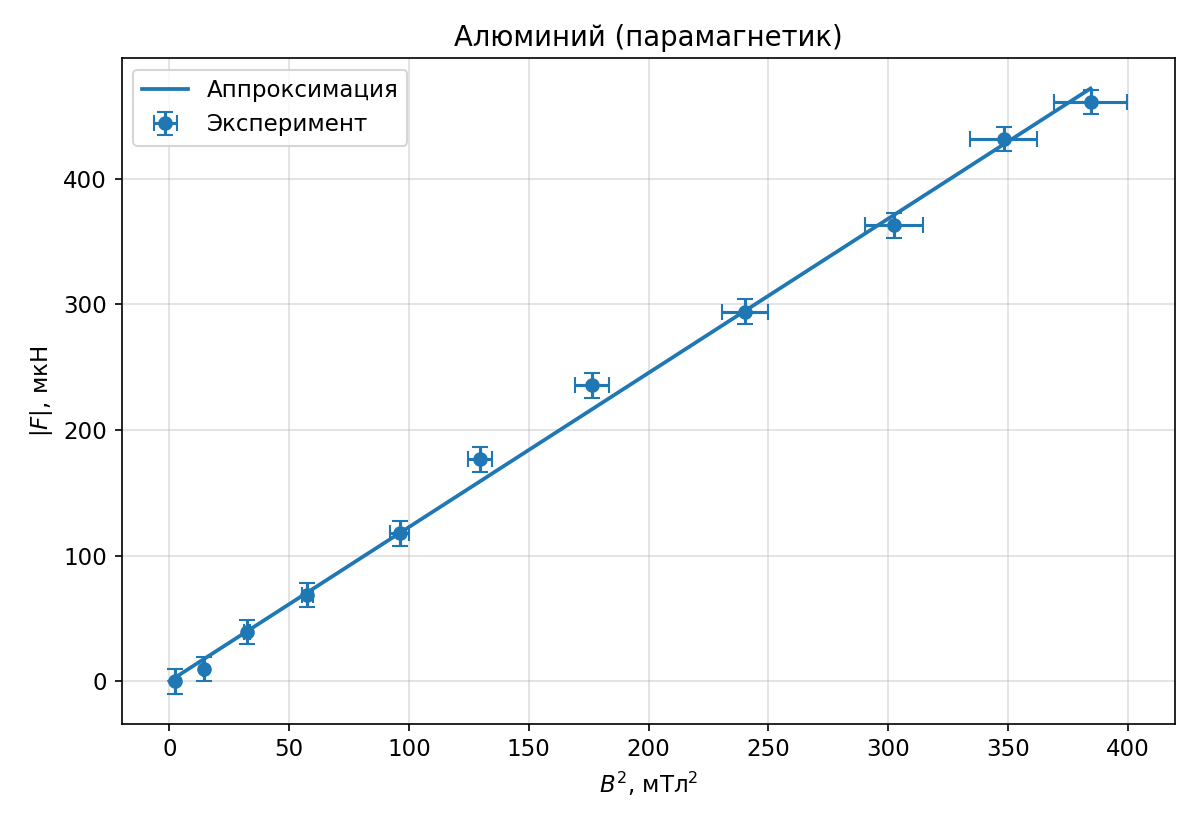
\includegraphics[width=0.82\textwidth]{plot_3_4_1_Al.png}
		\caption{Алюминий: зависимость $|F|$ от $B^2$ с погрешностями}
		\label{fig:Al}
	\end{figure}
	
	\begin{figure}[H]
		\centering
		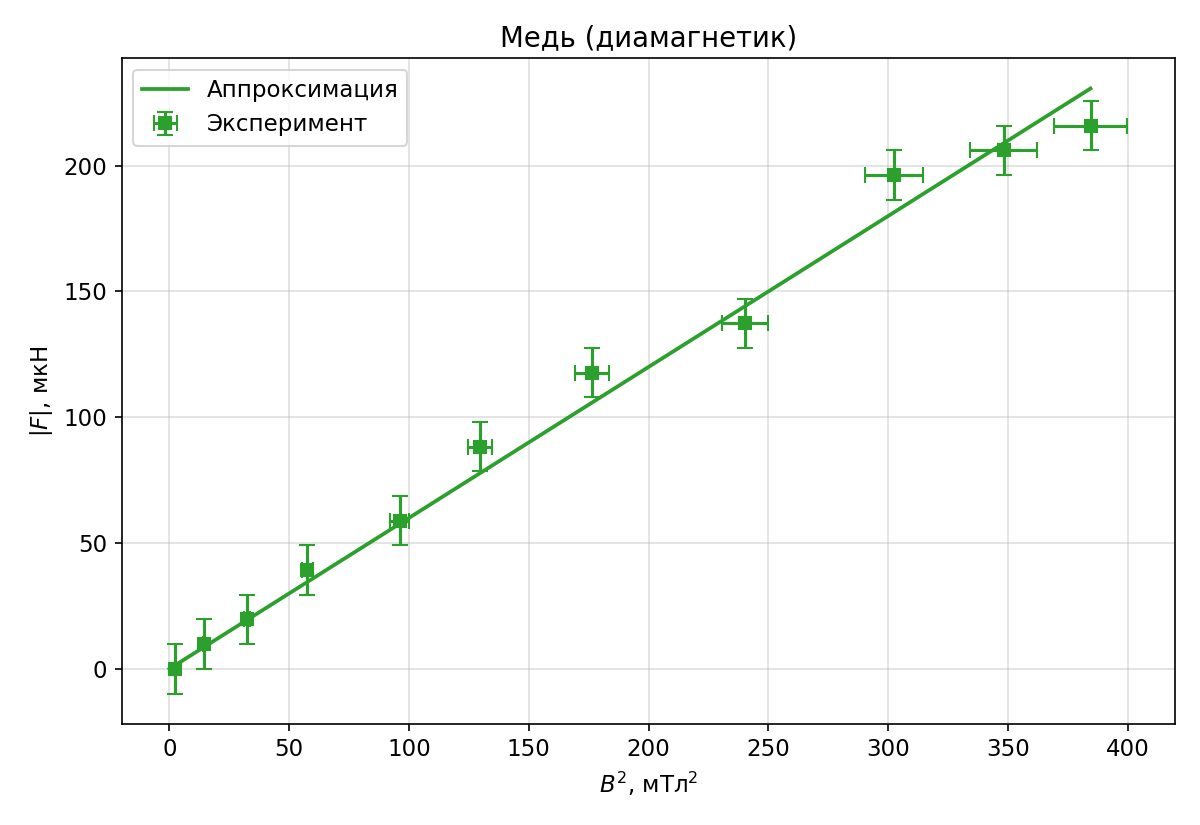
\includegraphics[width=0.82\textwidth]{plot_3_4_1_Cu.png}
		\caption{Медь: зависимость $|F|$ от $B^2$ с погрешностями}
		\label{fig:Cu}
	\end{figure}
	
	\subsection{Оценка погрешностей}
	Источники: $\delta B/B = 2\%$ (систематика калибровки), $\delta m = 1$~мг, $\delta r = 0{,}1$~мм ($\delta S/S = 4\%$). Статистическая погрешность наклона из МНК: $\sim 4\%$. Суммарная погрешность $k$ (с учётом $4\%$ от поля): $5{,}7\%$. Погрешность $\chi$ (с учётом $\delta S/S$): $\approx 7{,}0\%$. Итоговые значения сведены в табл.~\ref{tab:sum1}.
	
	\begin{table}[H]
		\centering
		\caption{Сводные результаты 3.4.1}
		\label{tab:sum1}
		\begin{tabular}{lcc}
			\toprule
			Величина & Al (парамагнетик) & Cu (диамагнетик) \\
			\midrule
			$k$, Н/Тл$^2$ & $(1{,}228 \pm 0{,}051)\cdot 10^{-3}$ & $(6{,}00 \pm 0{,}28)\cdot 10^{-4}$ \\
			$\chi$        & $(3{,}93 \pm 0{,}23)\cdot 10^{-5}$   & $-(1{,}92 \pm 0{,}12)\cdot 10^{-5}$ \\
			Табличное $\chi$ & $2{,}2\cdot10^{-5}$              & $-9{,}6\cdot10^{-6}$ \\
			\bottomrule
		\end{tabular}
	\end{table}
	
	\subsection{Выводы}
	Получены значения магнитной восприимчивости алюминия ($\chi > 0$) и меди ($\chi < 0$), по порядку величины согласующиеся с табличными. Расхождение по абсолютной величине объясняется неоднородностью поля в зазоре и возможным присутствием примесей.
	
	\newpage
	
	% ============================================================
	%  РАБОТА 3.4.2
	% ============================================================
	\section{Лабораторная работа 3.4.2. Закон Кюри--Вейсса}
	
	\subsection{Аннотация}
	Цель работы: изучение температурной зависимости магнитной восприимчивости гадолиния выше точки Кюри, проверка закона Кюри--Вейсса и определение парамагнитной точки Кюри $\Theta_p$.
	
	\subsection{Теоретические сведения}
	Выше точки Кюри ферромагнетик переходит в парамагнитное состояние, в котором восприимчивость подчиняется закону Кюри--Вейсса:
	\begin{equation}
		\chi = \frac{C}{T - \Theta_p}.
	\end{equation}
	Индуктивность катушки с образцом пропорциональна магнитной проницаемости среды, поэтому $\chi \propto \tau^2 - \tau_0^2$, где $\tau$~--- период $LC$-автогенератора с образцом, $\tau_0$~--- без образца. Отсюда
	\begin{equation}
		\frac{1}{\tau^2 - \tau_0^2} \propto T - \Theta_p.
	\end{equation}
	График $1/(\tau^2-\tau_0^2)$ от $T$ в парамагнитной области должен быть линейным; точка пересечения с осью абсцисс даёт $\Theta_p$.
	
	\subsection{Методика измерений}
	Образец гадолиния помещён в катушку $LC$-автогенератора; температура регулируется термостатом и контролируется медно-константановой термопарой. Период измеряется частотомером; $\tau_0 = 8{,}252$~мкс. Диапазон температур 14--40\,°C. Погрешности: $\delta T = 0{,}5$~°C, $\delta\tau = 0{,}001$~мкс, $\delta\tau_0 = 0{,}001$~мкс.
	
	\subsection{Результаты измерений}
	В табл.~\ref{tab:curie} приведены измеренные значения $\tau(T)$ и вычисленная величина $y = 1/(\tau^2 - \tau_0^2)$. Погрешность $\delta y$ вычислена по формуле производной.
	
	\begin{table}[H]
		\centering
		\caption{Данные для гадолиния}
		\label{tab:curie}
		\begin{tabular}{cccc}
			\toprule
			$T \pm \delta T$, °C & $\tau$, мкс & $y = 1/(\tau^2 - \tau_0^2)$, мкс$^{-2}$ & $\delta y / y$, \% \\
			\midrule
			$14{,}2 \pm 0{,}5$ & 10.4082 & $0{,}02485 \pm 0{,}00001$ & 0{,}05 \\
			$16{,}0 \pm 0{,}5$ & 9.958738 & $0{,}03217 \pm 0{,}00002$ & 0{,}06 \\
			$18{,}0 \pm 0{,}5$ & 9.776049 & $0{,}03640 \pm 0{,}00002$ & 0{,}07 \\
			$20{,}0 \pm 0{,}5$ & 9.53297  & $0{,}04389 \pm 0{,}00003$ & 0{,}08 \\
			$22{,}0 \pm 0{,}5$ & 9.189143 & $0{,}06118 \pm 0{,}00007$ & 0{,}11 \\
			$24{,}0 \pm 0{,}5$ & 8.778818 & $0{,}11145 \pm 0{,}00022$ & 0{,}20 \\
			$26{,}0 \pm 0{,}5$ & 8.62145  & $0{,}16041 \pm 0{,}00040$ & 0{,}25 \\
			$28{,}0 \pm 0{,}5$ & 8.535055 & $0{,}21045 \pm 0{,}00065$ & 0{,}31 \\
			$30{,}0 \pm 0{,}5$ & 8.485958 & $0{,}25536 \pm 0{,}00090$ & 0{,}35 \\
			$32{,}0 \pm 0{,}5$ & 8.452457 & $0{,}29864 \pm 0{,}00118$ & 0{,}40 \\
			$34{,}0 \pm 0{,}5$ & 8.426839 & $0{,}34292 \pm 0{,}00150$ & 0{,}44 \\
			$36{,}0 \pm 0{,}5$ & 8.406604 & $0{,}38827 \pm 0{,}00187$ & 0{,}48 \\
			$38{,}0 \pm 0{,}5$ & 8.392871 & $0{,}42648 \pm 0{,}00222$ & 0{,}52 \\
			$40{,}0 \pm 0{,}5$ & 8.38079  & $0{,}46683 \pm 0{,}00261$ & 0{,}56 \\
			\bottomrule
		\end{tabular}
	\end{table}
	
	\subsection{Обработка результатов}
	Закон Кюри--Вейсса справедлив только в парамагнитной области. Точка Кюри для гадолиния $\approx 20$~°C, поэтому точки при $T < 22$~°C (в области фазового перехода) из фита исключены. Линейная аппроксимация проведена взвешенным МНК по 10 точкам ($T \ge 22$~°C):
	\begin{align}
		b &= (2{,}423 \pm 0{,}007)\cdot 10^{-2}\ \text{мкс}^{-2}\cdot\text{°C}^{-1},\\
		a &= -(4{,}716 \pm 0{,}015)\cdot 10^{-1}\ \text{мкс}^{-2}.
	\end{align}
	Тогда
	\[
	\Theta_p = -\frac{a}{b} = (19{,}47 \pm 0{,}08)\ \text{°C}.
	\]
	
	\begin{figure}[H]
		\centering
		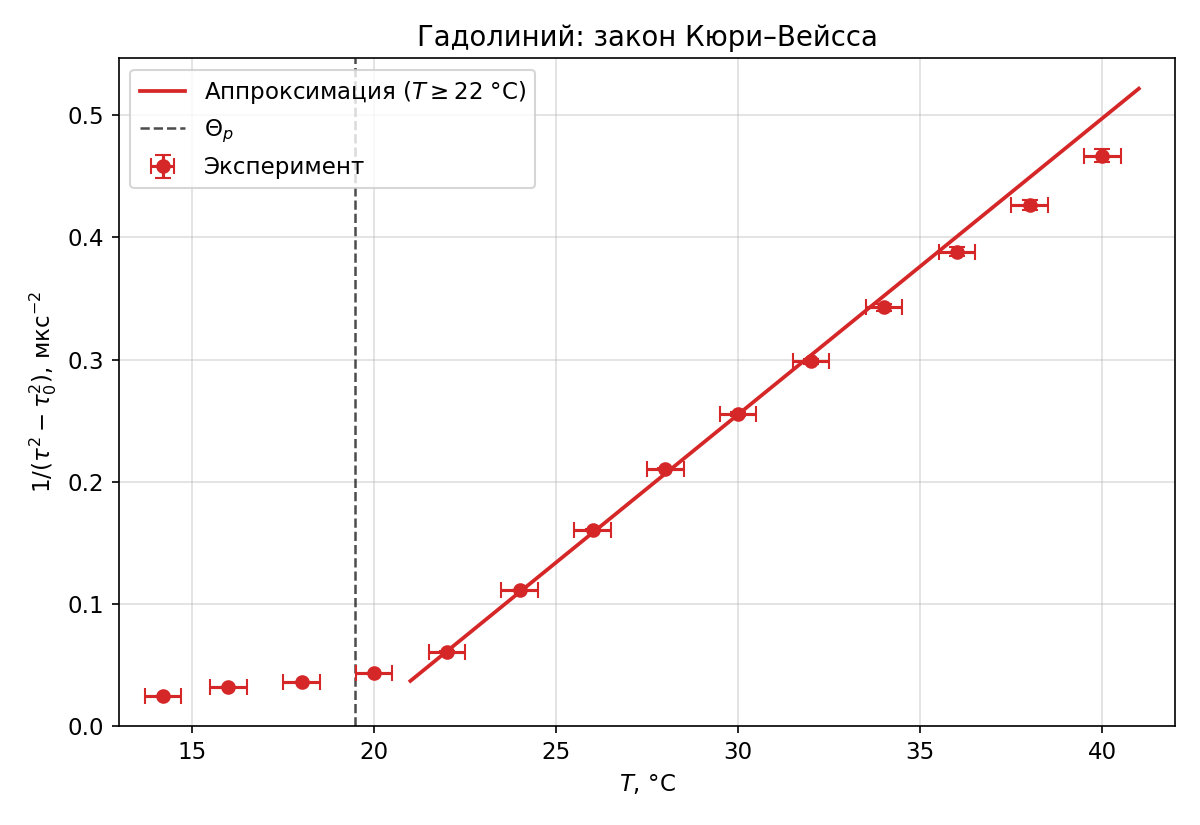
\includegraphics[width=0.88\textwidth]{plot_3_4_2.png}
		\caption{Зависимость $1/(\tau^2-\tau_0^2)$ от $T$ для гадолиния. Штриховая линия~--- $\Theta_p$}
		\label{fig:curie}
	\end{figure}
	
	\paragraph{Замечание о $\chi^2/ndf$.} Значение $\chi^2/ndf = 18{,}8$ кажется большим. Это связано с тем, что статистические погрешности $\delta y$ (обусловленные точностью частотомера $\delta\tau = 0{,}001$~мкс) очень малы. На таком уровне точности проявляется систематическое отклонение реальной зависимости от идеального закона Кюри--Вейсса: вблизи $T_c \approx 20$~°C закон нарушается, а на верхней границе диапазона сказывается зависимость параметров установки от температуры.
	
	\subsection{Оценка погрешностей}
	Прямые измерения: $\delta T = 0{,}5$~°C, $\delta\tau = 0{,}001$~мкс, $\delta\tau_0 = 0{,}001$~мкс. Погрешность $y$ вычислена по формуле производной. Погрешность $\Theta_p$:
	\[
	\delta\Theta_p = \Theta_p\sqrt{(\delta a/a)^2 + (\delta b/b)^2}
	\approx 19{,}47\cdot\sqrt{(0{,}0032)^2 + (0{,}0028)^2} \approx 0{,}08\ \text{°C}.
	\]
	Погрешность температуры даёт аддитивный сдвиг по оси абсцисс.
	
	\subsection{Выводы}
	Измерена температурная зависимость магнитной восприимчивости гадолиния. Показано, что в парамагнитной области ($T \ge 22$~°C) выполняется закон Кюри--Вейсса. Определена парамагнитная точка Кюри $\Theta_p = (19{,}47 \pm 0{,}08)$~°C, что согласуется с табличным значением $\approx 20$~°C. Отклонение от линейности при $T < 22$~°C соответствует переходу в ферромагнитное состояние.
	
	\appendix
	\section{Графики}
	\begin{figure}[H]\centering
		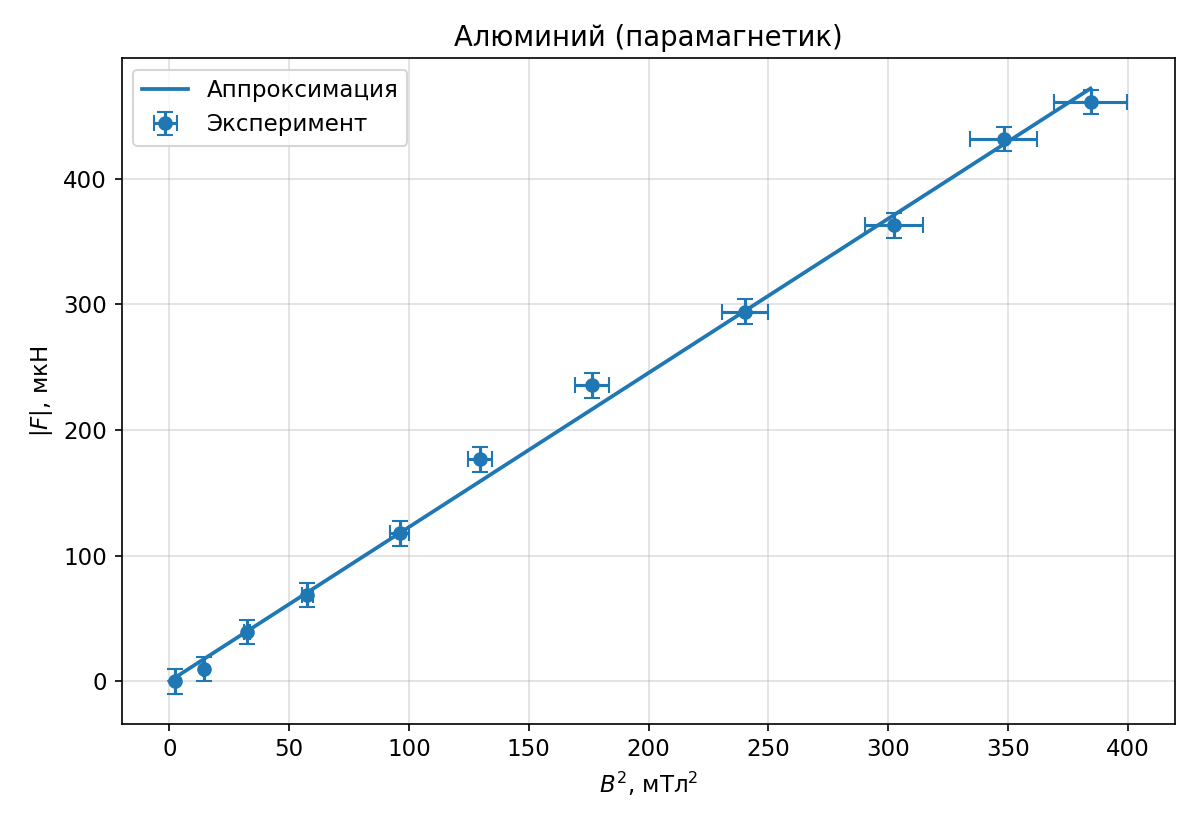
\includegraphics[width=0.82\textwidth]{plot_3_4_1_Al.png}
		\caption{3.4.1: алюминий}
	\end{figure}
	\begin{figure}[H]\centering
		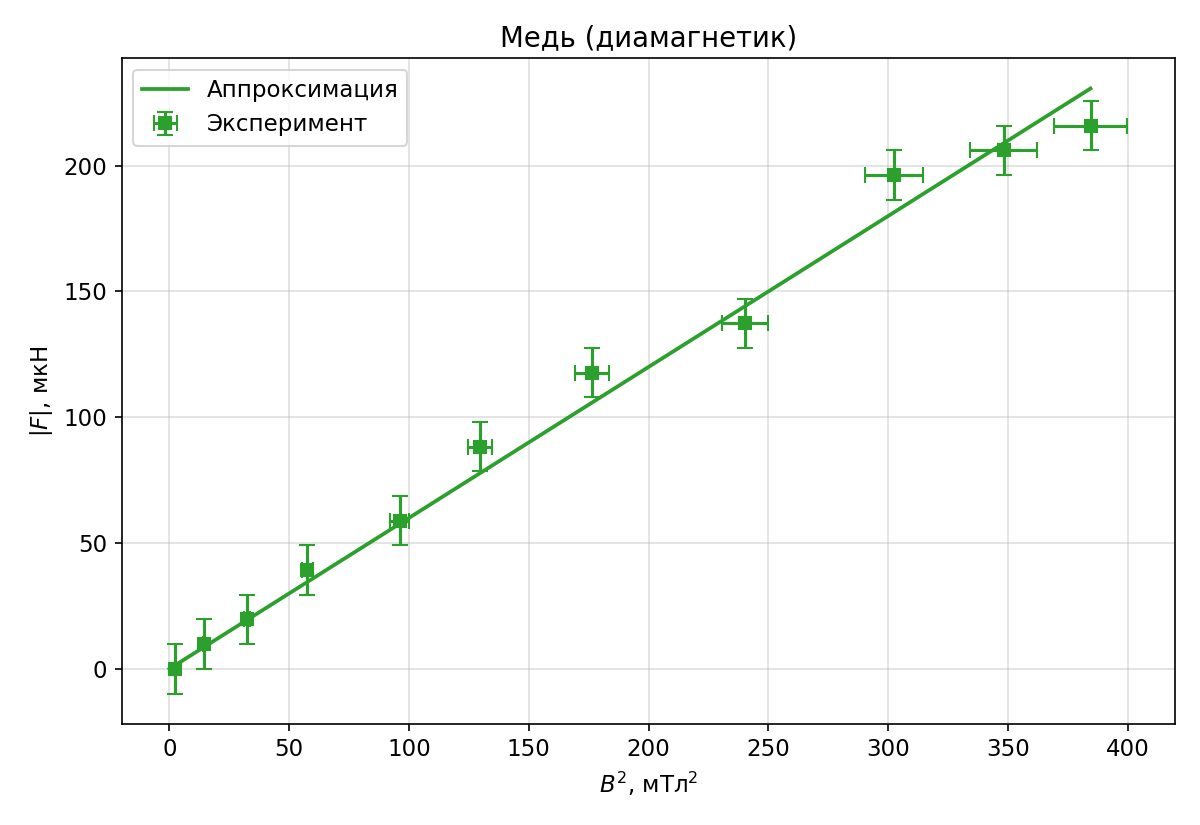
\includegraphics[width=0.82\textwidth]{plot_3_4_1_Cu.png}
		\caption{3.4.1: медь}
	\end{figure}
	\begin{figure}[H]\centering
		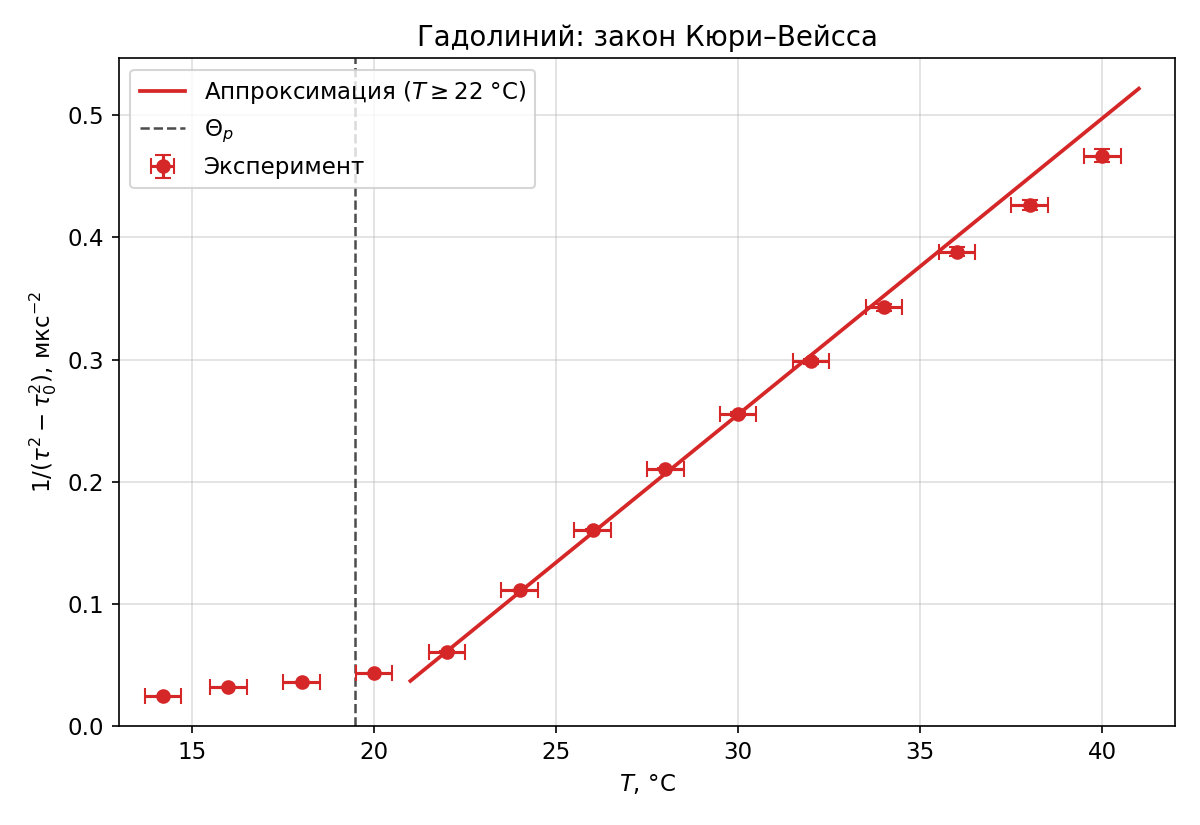
\includegraphics[width=0.88\textwidth]{plot_3_4_2.png}
		\caption{3.4.2: гадолиний}
	\end{figure}
	
\end{document}